\subsection{ Discretization with Contact Segments}
The discretization of the contact interface by segments as described for the linear case in Simo, Wriggers, Taylor (1985) or for large deformations in Papadopoulos, Taylor (1992) leads to a special mixed formulation. Following Simo, Wriggers, Taylor (1985) we state the interpolation of the gap function $ g_{N} $ and its variation $ \delta g_{N} $ for a geometrically linear setting as follows

\begin{equation}
\label{eqn:4.65}
g_{N}=\left[\mathbf{u}^{1}(\xi)-\mathbf{u}^{2}(\xi)\right] \cdot \mathbf{n}(\xi) \quad \delta g_{N}=\left[\boldsymbol{\eta}^{1}(\xi)-\boldsymbol{\eta}^{2}(\xi)\right] \cdot \mathbf{n}(\xi)
\end{equation}

These interpolations are applied within a segement which is defined by the edge nodes $ \mathbf{x}_{2}^{A} $ and the projections onto the other surface $ \overline{\mathbf{x}}^{{A}} $, see Figure \ref{fig4:7}.
\begin{figure}
    \centering
    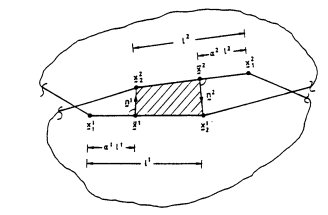
\includegraphics{Figure2/Chap4/fig7.png}
    \caption{Contact segment element}
   \label{fig4:7}
\end{figure}

Within this segment the displacement field and its variation is given as
\begin{equation}
\label{eqn:4.66}
\mathbf{u}^{\gamma}(\xi)=(1-\xi) \overline{\mathbf{u}}^{\gamma}+\xi \mathbf{u}_{2}^{\gamma} \quad \boldsymbol{\eta}^{\gamma}(\xi)=(1-\xi) \overline{\boldsymbol{\eta}}^{\gamma}+\xi \boldsymbol{\eta}_{2}^{\gamma}
\end{equation}
or the surface of the body $ \mathcal{B}^{\gamma}, \gamma=1,2 $. For the perturbed Lagrangian approach $ (38) $ the contact contributions take the form

\begin{equation}
\label{eqn:4.67}
\begin{aligned} \int_{\Gamma_{c}} \lambda_{N} \delta g_{N} d \Gamma &=\sum_{s=1}^{n_{s e g}} \int_{\Gamma_{s}} \lambda_{N} \delta g_{N} d \Gamma \\ \int_{\Gamma_{c}}\left(-\frac{\lambda_{N}}{\epsilon_{N}}+g_{N}\right) \delta \lambda_{N} d \Gamma &=\sum_{s=1}^{n_{s e g}} \int_{\Gamma_{s}}\left(-\frac{\lambda_{N}}{\epsilon_{N}}+g_{N}\right) \delta \lambda_{N} d \Gamma=0 \end{aligned} 
\end{equation}
where the latter equation can be solved for $ \lambda_{N} $ directly. With the interpolations $ (65) $ and assuming a constant contact pressure $ \lambda_{N} $ within the segment, $ \lambda_{N}=\bar{\lambda}_{N}=C O N S T . $, we obtain for the segment $ \Gamma_{s} $
\begin{equation}
\label{eqn:4.68}
\begin{aligned} \int_{\Gamma_{s}} \lambda_{N} \delta g_{N} d \Gamma &=\bar{\lambda}_{N} \int_{0}^{1}\left[\boldsymbol{\eta}^{1}(\xi)-\boldsymbol{\eta}^{2}(\xi)\right] \cdot \mathbf{n}(\xi)\left\|\frac{d \Gamma}{d \xi}\right\| d \xi \\ \int_{\Gamma_{s}}\left(-\frac{\lambda_{N}}{\epsilon_{N}}+g_{N}\right) \delta \lambda_{N} d \Gamma \Longrightarrow \bar{\lambda}_{N} &=\frac{\epsilon_{N}}{L_{s}} \int_{0}^{1}\left[\mathbf{u}^{1}(\xi)-\mathbf{u}^{2}(\xi)\right] \cdot \mathbf{n}(\xi)\left\|\frac{d \Gamma}{d \xi}\right\| d \xi \end{aligned}
\end{equation}